% Options for packages loaded elsewhere
\PassOptionsToPackage{unicode}{hyperref}
\PassOptionsToPackage{hyphens}{url}
\documentclass[]{article}
\usepackage{graphicx}
\usepackage{flafter}
\usepackage{svg}
\usepackage[section]{placeins}
\usepackage{amsmath}
\usepackage[ruled]{algorithm2e}
\usepackage[a4paper, portrait, margin=1in]{geometry}
\makeatother
\setlength{\emergencystretch}{3em} % prevent overfull lines
\providecommand{\tightlist}{%
  \setlength{\itemsep}{0pt}\setlength{\parskip}{0pt}}
\usepackage{bookmark}
\IfFileExists{xurl.sty}{\usepackage{xurl}}{} % add URL line breaks if available
\urlstyle{same}
\hypersetup{
  pdftitle={dissertation},
  hidelinks,
  pdfcreator={cassette :)}}

\title{An Examination of Isosurface Extraction for Terrain in Videogames}
\author{Cassette Costen}
\date{2026}

\begin{document}
\maketitle


\begin{center}
    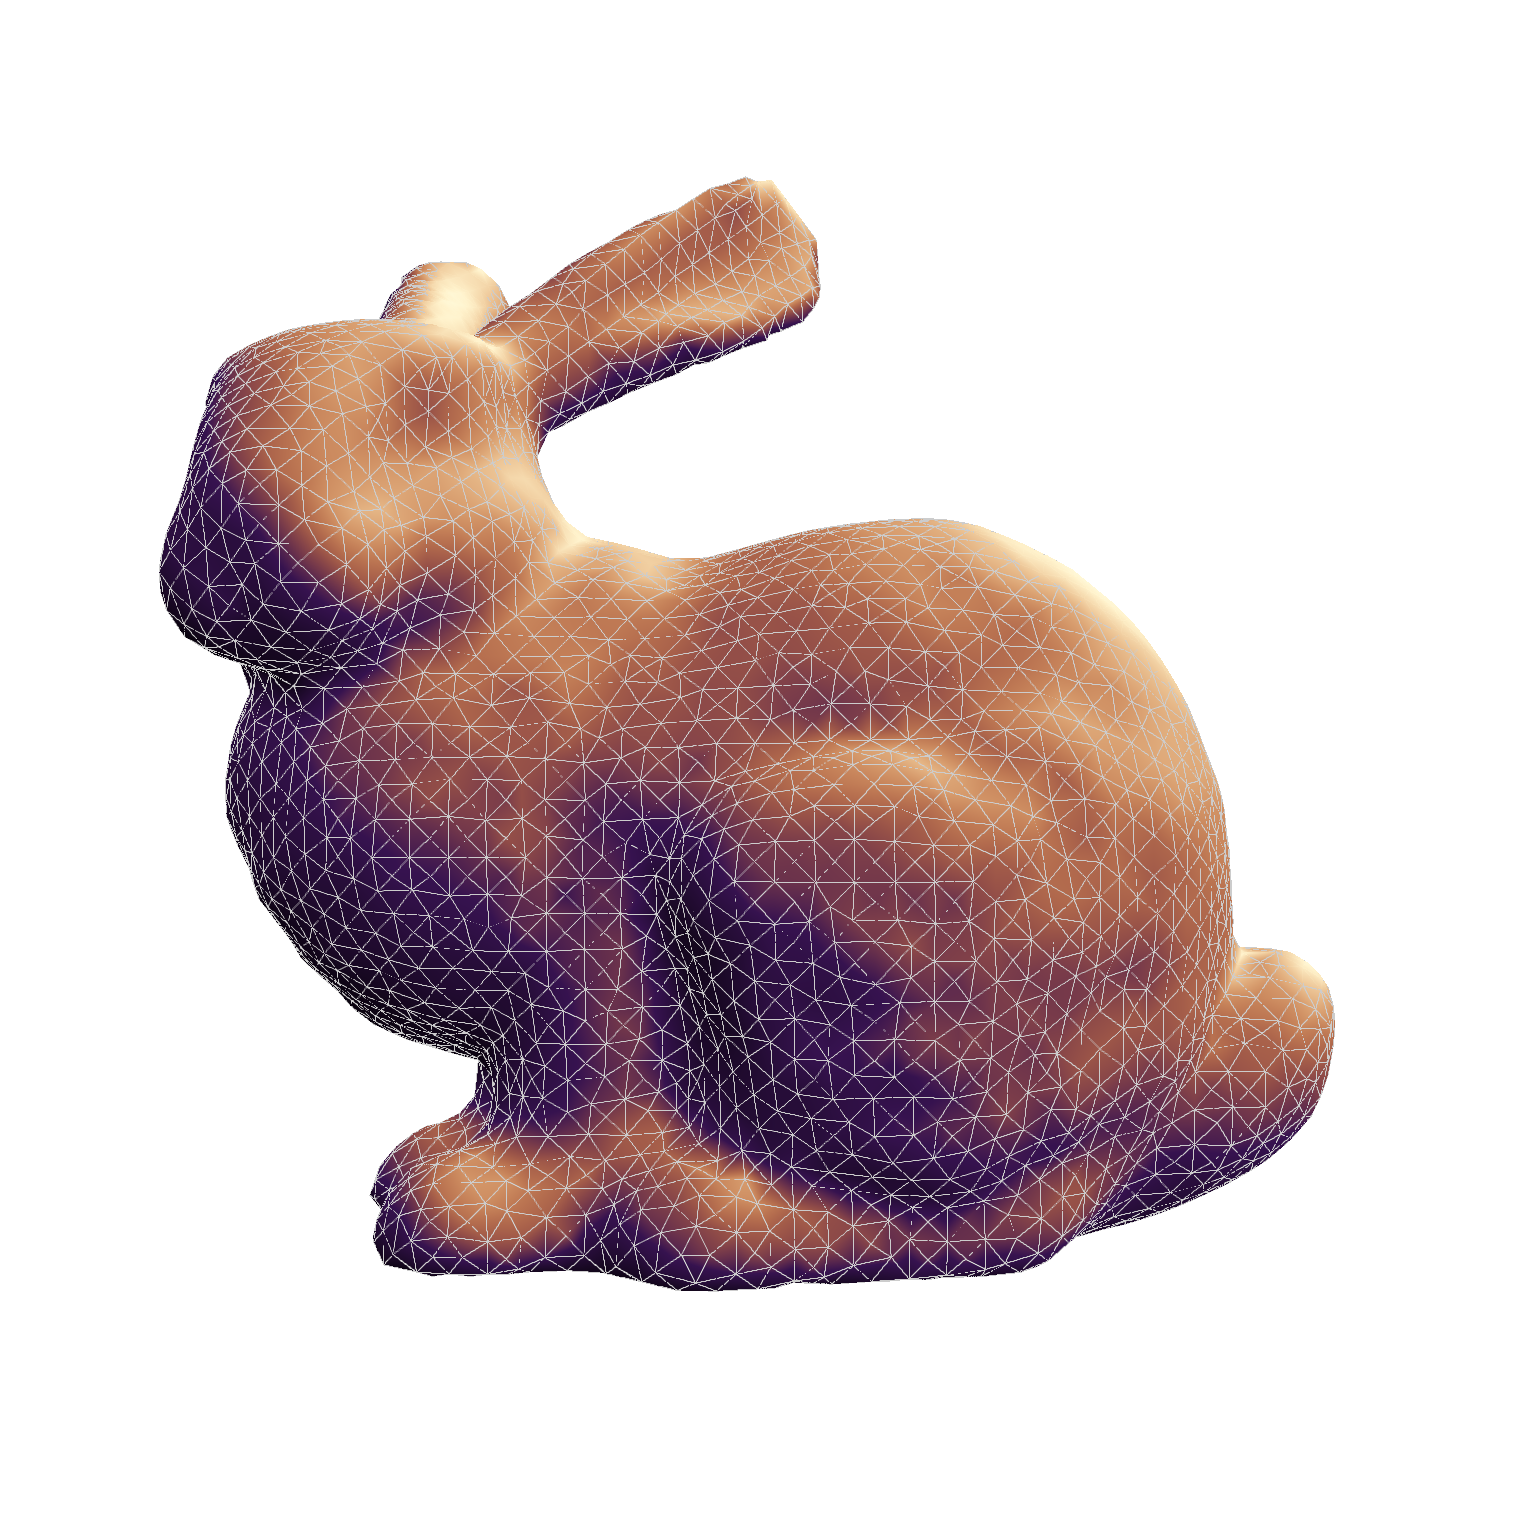
\includegraphics[width=\textwidth]{header.png}
\end{center}

\FloatBarrier

\newpage

\section{Introduction}\label{introduction}

This paper compares several variations of the marching tetrahedra approach to extraction of isosurfaces from 3-dimensional scalar functions. It evaluates the demonstrated algorithms for their fitness specifically as applied to real-time procedural mesh generation for terrain in videogames, in scenarios where simple heightmaps are insufficient. Procedural mesh generation presents several challenges, particularly for use in videogames. Resulting meshes must be visually complete and water-tight without additional human intervention, must be minimal in triangle count to meet real-time performance targets, and must produce sensible results when shaded with common techniques. The mesh generation itself must be highly optimised for both performance and memory consumption - with particular consideration given to minimising startup time.

Literature in relation to relevant isosurface extraction methods is examined, and the landmark \textquotesingle regularised marching tetrahedra\textquotesingle{} algorithm presented by Treece et. al. (1999) is implemented. An alternative arrangement of the tetrahedral lattice, and an alternative mesh simplification algorithm are demonstrated and the impact of these variations is examined with regard to the computation time, triangle count and mean aspect ratio, and perceived visual quality of resulting meshes. This paper aims to detail the state of isosurface extraction techniques and explore further opportunities specifically regarding use in videogame terrain generation.

\subsection{Technical Considerations}\label{technical-considerations}

For real-time rendering applications such as videogames, triangle counts should be reduced where possible to minimise GPU utilisation. Since terrain meshes often take on organic forms as a result of procedural noise, some even being grown using evolutionary algorithms (Raffe et al., 2012), they can benefit greatly from regularisation techniques which are able to distribute triangles and eliminate small faces. Extremely small or narrow faces which often result from isosurface extraction algorithms are wasteful both due to overall triangle count, and as a result of overdraw. Nearly all modern graphics acceleration hardware shade pixels in $2\times2$ quads to facilitate calculation of derivatives of per-pixel variables such as UV coordinates (Penner and Engel, 2011). Overdraw occurs when wasted work is performed due to a triangle only covering a portion of a quad, resulting in pixels being shaded many more times than is necessary and contributing to worse performance. This scenario becomes very frequent when rendering meshes with many highly elongated or tiny triangles.

The presence of tiny or elongated triangles in an organic mesh also results in shading irregularities which significantly degrade the appearance of geometry shaded using interpolated surface normals (such as Phong shading). See Fig. \ref{fig:eviltriangles} and Fig. \ref{fig:nicetriangles} for an illustration of this effect.

\begin{figure}[htb]
    \centering
    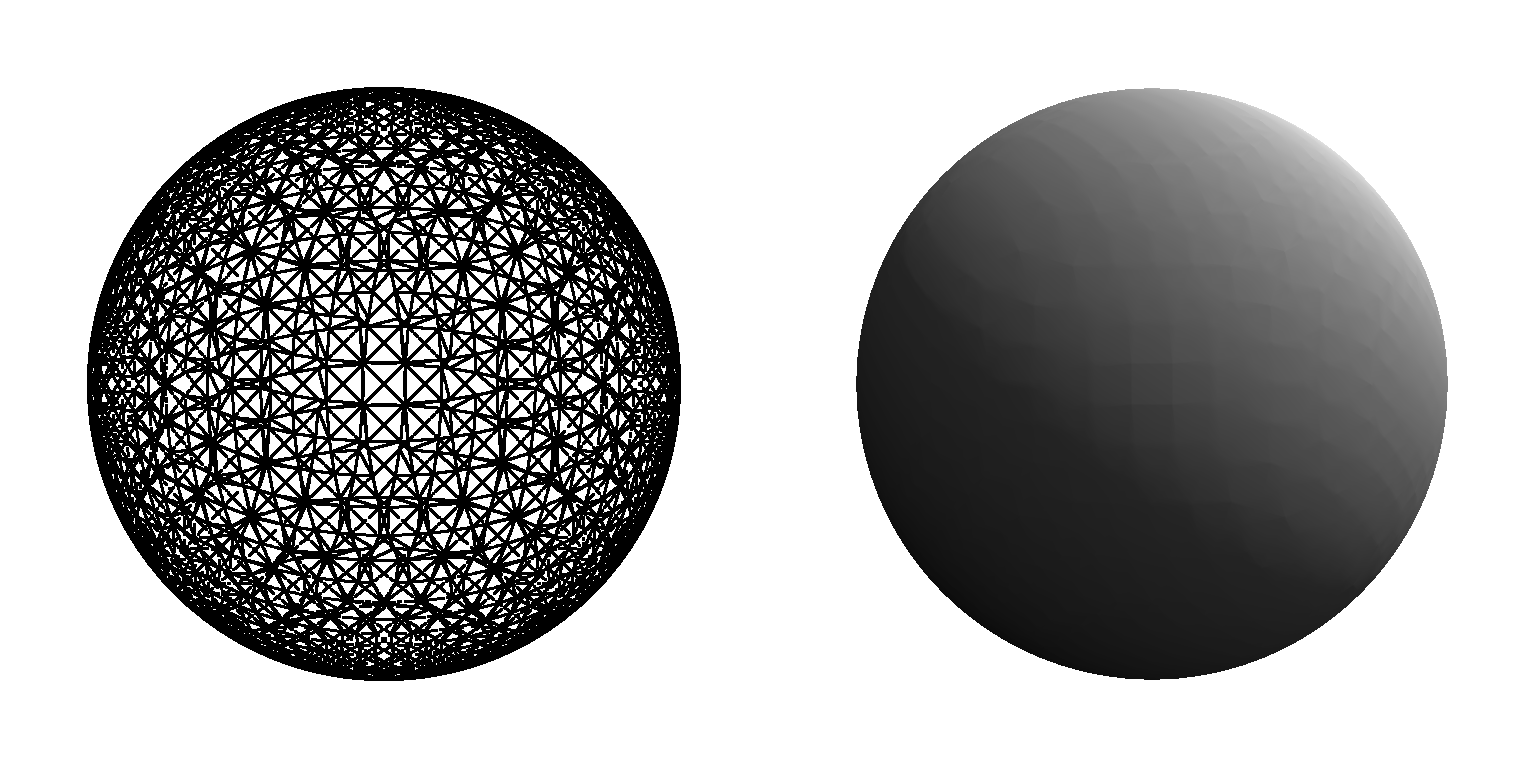
\includegraphics[width=0.75\textwidth]{evil triangles.png}
    \caption{A sphere mesh with many highly elongated triangles, resulting in uneven shading.}
    \label{fig:eviltriangles}
\end{figure}

\begin{figure}[htb]
    \centering
    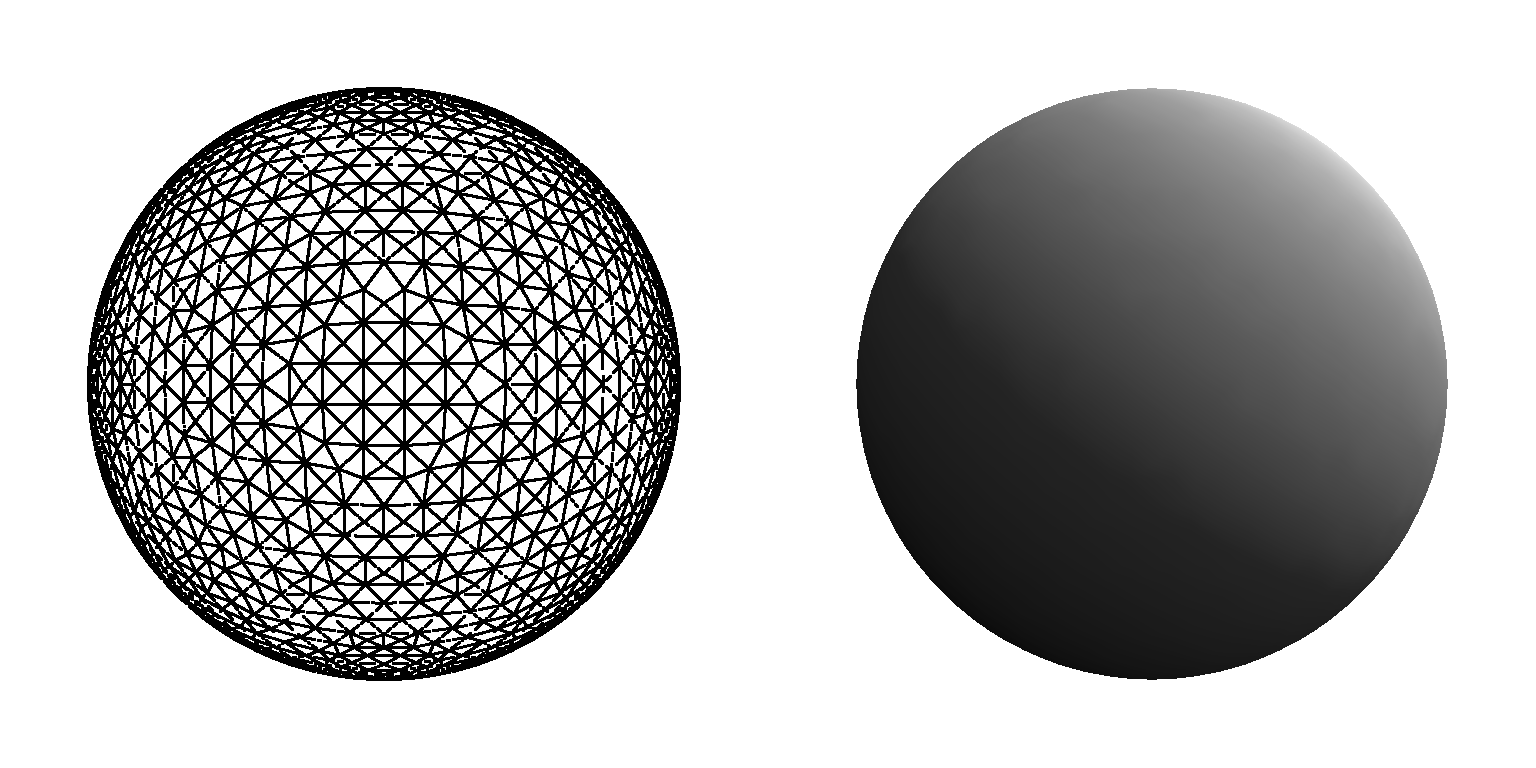
\includegraphics[width=0.75\textwidth]{nice triangles.png}
    \caption{A regularised sphere mesh, resulting in even, smooth shading.}
    \label{fig:nicetriangles}
\end{figure}

\FloatBarrier

Ideally, all triangles in the resulting mesh should be equilateral, or as close to equilateral as possible to tile the surface, as this minimises the deviation in internal corner angles for the triangle and thus also minimises the appearance of shading anomalies. Tiling a surface with equilateral triangles also results in the most efficient filling of surface area, which significantly reduces work wasted due to overdraw as mentioned above. Within this paper, triangles being described as poor quality implies they are highly elongated or extremely small.

In addition to this, the performance of the isosurface extraction algorithm is of great importance. Many videogames involve procedurally generated terrain - often dynamic terrain modifiable by the player, such as in ASTRONEER (2016), which contains stylised, polygonal, continuously deformable terrain. In order to facilitate this, two considerations are made: first, that the algorithm should be capable of evaluating a usefully-sized volume of space within a typical game frame-time (1/60th of a second); second, that the algorithm should be capable of evaluating a larger volume as a series of smaller blocks if necessary. The first of these considerations must also make note of the startup time for the algorithm - an ideal implementation would keep existing memory allocated where practical, and give sufficient control to the developer to eliminate unnecessary re-evaluation of sampling data. The second consideration allows for staggering mesh computation over multiple frames or compute units, as well as avoiding re-computation of the entire sample space. Modifiable terrain is rarely altered in many places at once, and thus not all of the space must be re-tessellated for every modification.

Another key consideration for the algorithm is that it reliably produces manifold, closed geometry. A manifold implies a surface which does not intersect itself, where its surface is appears locally Euclidian at all points (Lee, 2012). Specifically this use case involves 2D manifold, or 2-manifold, embedded in a 3D space. For videogames, the manifoldness restriction produces a mesh which does not appear to cross itself - which would usually be considered non-physical and thus inappropriate for terrain - and which does not instantaneously invert its orientation; normal vectors must vary continuously across the surface. The restriction on being closed produces a mesh which has a defined inside and outside - as conveyed by the direction of the surface normal vectors - and which has no loose geometry or holes, except where the sample space being evaluated terminates. All of these conditions are necessary to produce geometry which may be perceived by players as physically solid, as single-sided holes, self-intersections, and surfaces viewable from a reverse angle - often referred to as \textquotesingle backfacing\textquotesingle, as the camera sees the back side of the face which is often culled for performance and may result in perceived mesh holes - all break the illusion of a solid object.

The final technical requirement is that the algorithm be able to produce a mesh directly from a given scalar function. This enables extraction of isosurfaces from procedural noise functions without need of an intermediate meshing process, significantly reducing the computational cost of the algorithm. While techniques for re-contouring or simplifying existing meshes have been previously explored in research such as Cignoni et al., (1998) and applied to isosurface extraction, they are not entirely appropriate for such high-performance applications when compared with techniques which produce simplified meshes directly.

\newpage

\section{Literature Review}\label{literature-review}

\subsection{Isosurfaces}\label{isosurfaces}

Isosurface extraction refers to the construction of a geometric surface in $n$-dimensional space filled with a scalar field, such that all points on that surface have the same value in the scalar field. For example, for a scalar field defined by the formula $\sqrt{x^2 + y^2}$, the manifold representing an isovalue of 1 would be a circle, of radius 1, centered on the origin (see Fig. \ref{fig:circlemanifold}).

\begin{figure}[htb]
    \centering
    \includesvg[inkscapelatex=false,width=0.75\textwidth]{circle 1d manifold.svg}
    \caption{A 1-manifold representing the isosurface defined by $f(x, y) = \sqrt{x^2 + y^2}$ and isovalue 1.}
    \label{fig:circlemanifold}
\end{figure}

\FloatBarrier

A significant volume of research has been conducted on the subject of isosurface extraction, predominantly for the purpose of visualising medical imaging results. An early example considers the problem of rendering CT scan results into smooth 3D surfaces, without large computational or storage costs, by bypassing the isosurface representation and producing a shaded image directly from the \textquotesingle cuberille\textquotesingle{} voxel data (Chen et al., 1985).

\subsection{Marching Cubes}\label{marching-cubes}

The most well-known algorithm for isosurface extraction is the marching cubes algorithm, presented in Lorensen and Cline (1998). Also developed for medical imaging purposes, marching cubes produces triangle geometry for small blocks of the sample space one-by-one, and then \emph{marches} to the next block. Each block is evaluated according to whether each corner of the currently considered cube is inside or outside the isosurface (that is to say, whether the value at each corner is less than or greater than the chosen isovalue); the set of eight Boolean corner states is then used to index into a table of predefined geometries, shown in Fig. \ref{fig:mcconfigs}. The table of potential geometry configurations is quite large; initially on the order of 256, it can be reduced to just 14 unique cases via symmetry and rotations. Each vertex position is then interpolated along their owning edge such that they lie on the isosurface.

\begin{figure}[htb]
    \centering
    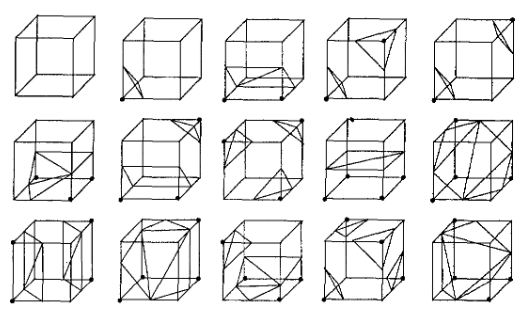
\includegraphics[width=0.75\textwidth]{marching cubes configurations.png}
    \caption{The 14 unique triangulations used by the marching cubes algorithm (Shu et al., 1995).}
    \label{fig:mcconfigs}
\end{figure}

\FloatBarrier

This divide-and-conquer approach simplifies the problem and enables parallelisation as the individual cubes of the sample space are entirely independent and disjointed. That said, there is some shared computation on the boundary between two cubes, and the parallel approach requires vertices on the boundary to be merged later to avoid unnecessarily high storage cost.

However, the original marching cubes algorithm has ambiguous geometry for some configurations (Chan and Purisima, 1998) where faces of the cube include pairs of diagonally opposed states, shown in Fig. \ref{fig:mcambiguity}. Several improvements to the original marching cubes algorithm have been proposed to address this, but which involve additional tests and thus increase the computational cost (Zhou et al., 1995; Gallagher and Nagtegaal, 1989). One example of this considers bilinear interpolation across the ambiguous face - as opposed to simple linear interpolation along the cube edges - and determining which pairs of candidate vertices are sensibly joined by a hyperbolic arc in the bilinear interpolant. This is then used to select between potential triangulations of the cube (Nielson and Hamann, 1991).

\begin{figure}[htb]
    \centering
    \includesvg[inkscapelatex=false,width=0.75\textwidth]{marching cubes ambiguity.svg}
    \caption{Illustration of the ambiguity problem with marching cubes. Without additional information, it cannot be determined which of the two triangulations is appropriate, which results in holes between cubes when extended into 3D.}
    \label{fig:mcambiguity}
\end{figure}

\FloatBarrier

The marching cubes algorithm also produces a large number of triangles, many of which are of poor quality, which results in higher storage and rendering costs and a lower shading quality. This is of critical concern for videogames, since the visual presentation of the mesh to the player and the performance cost of rendering that mesh are of paramount importance.

Marching cubes has been the foundation of much isosurface extraction research, including extending the principle of axis-aligned marching isosurface extraction into higher dimensions. Castelo et al. (2024) present a generalised marching hypercubes algorithm which is able to
extract any $n$-dimensional manifold from a $p$-dimensional sample space, for any $n < p$.

\subsection{Marching Tetrahedra}\label{marching-tetrahedra}

The marching tetrahedra algorithm is a variation of marching cubes first presented by Payne and Toga (1990) which eliminates the ambiguity problem as a result of reducing the number of corners involved in a single primitive from 4 - in the case of a square cube face; to 3 - in the case of a triangular tetrahedron face (Zhou et al., 1995). At the same time, this reduces the number of configurations per cell to just 16, or 3 when considering symmetry and rotations. These per-tetrahedron configurations consist of only 0, 1, or 2 triangles each, and are shown in Fig. \ref{fig:mtconfigs}.

\begin{figure}[htb]
    \centering
    \includesvg[inkscapelatex=false,width=0.75\textwidth]{marching tetrahedra triangulations.svg}
    \caption{The unique configurations for a tetrahedral cell. Note that the fourth case shown is technically an inversion of the second case, meaning that only three unique cases exist, only two of which contain geometry.}
    \label{fig:mtconfigs}
\end{figure}

\FloatBarrier

When tessellating 3-dimensional space with tetrahedra, the arrangement of those tetrahedra must be considered. Most tessellations work around an orthogonal cubic grid, in order to integrate well with typical voxel data, such as that from CT scans. The three simplest arrangements are simple cubic (!DIAGRAM!), face-centered (!DIAGRAM!), and body-centered (!DIAGRAM!). It has been demonstrated that the body-centered lattice tessellation contains tetrahedra which have edge length ratios closest to 1, meaning they produce triangles closest to equilateral; this tessellation also has a higher sampling efficiency than other arrangements (Chan and Purisima, 1998; Chan and Purisima, 1998 (2)), hence many MT implementations use this arrangement.

However, marching tetrahedra generally produces worse meshes than marching cubes (Treece, Prager, and Gee, 1999) with a larger number of tiny or elongated triangles, which are undesirable. As such, both algorithms demand a simplification or regularisation mechanism to improve the final mesh. Simplification methods are discussed in more detail below.

\subsection{Regularised Marching Tetrahedra}\label{regularised-marching-tetrahedra}

RMT, presented by Treece, Prager, and Gee (1999), improves the marching tetrahedra algorithm by integrating the simplification process with the geometry generation process itself. RMT performs an intermediate vertex clustering procedure, eliminating the need for an expensive edge-collapse algorithm to be applied afterwards, and taking advantage of the topological context which is only available during geometry generation itself.

Each sample point is first determined to be either inside or outside the isosurface, and candidate vertices are positioned along edges which connect sample points, using interpolation to align them with the isosurface, as with marching cubes. Then, candidate vertices are grouped
according to which sample point they are closest to. The connectivity of these vertices are considered, and a subset of them may be merged together into a single vertex. Consideration of the connectivity allows the merging process to preserve topological features, such as closed
surfaces, loops, or disconnected pieces. The triangle mesh is then constructed in a later step using the vertices computed previously, using the same per-tetrahedron table of possible geometries as the existing marching tetrahedra algorithm. At this step, triangles which contain more than one copy of the same vertex - and thus would be \textquotesingle degenerate\textquotesingle, having zero area - are discarded. The actual implementation is described in greater detail in section \ref{algorithm}.

This \textquotesingle integrated\textquotesingle{} clustering method has many benefits over performing a regularisation or simplification algorithm after geometry has been produced. Firstly, this reduces memory consumption - there is no need to store a large number of vertices and then reduce the number later, the number of vertices produced is small to begin with. Secondly, because the clustering procedure is localised around each sample point, the number of elements which can be merged is bounded to the number of edges connecting to neighbouring sample points (14), which means the integrated clustering method overall has a worst-case complexity of $O(n)$, where $n$ is the number of sample points being considered. This results in significantly faster computation on average compared to post-processed simplification methods, as well as placing an upper bound on computation time. Finally, the integrated clustering approach is able to take advantage of the available topology information. The algorithm only operates on a local set of points, and connectivity information is available for the whole set, which is not the case with post-processed clustering algorithms unless significant additional mesh analysis is performed. This information can be used to prevent merging of certain features which would alter the underlying topology of the mesh.

As a result the total number of vertices and triangles in the mesh is massively reduced (see section \ref{results-and-conclusions}), and tiny or highly elongated triangles are eliminated without the need for a separate simplification step after the geometry has been produced; at the same time topological details and mesh integrity are preserved.

The regularised marching tetrahedra algorithm has been further extended to process datasets where sample points may exist in more than two possible domains (Sun et al., 2023), allowing for the triangulation of complex surfaces between several regions of differing nature. This is achieved by labelling sample points with its presence inside and/or outside multiple isosurface regions, implementing additional checks during the vertex clustering process to prevent topology alteration across region boundaries, and expanding the table of tetrahedron triangulations to cover the additional cases. Multi-labeled RMT has strong applications in geological visualisation and medical imaging, although it is not applicable to the present task of mesh generation for videogames since it does not produce manifold, single-sided meshes (and is otherwise unnecessarily complex for this purpose).

\subsection{Other Isosurface Extraction Techniques}\label{other-isosurface-extraction-techniques}

Research has been conducted with the target of improving interactivity for isosurface extraction techniques. One implementation pre-processes datasets to extract a subset of which all selected cells - which, according to implementation, may be cubes, tetrahedra, or other - intersect the isovalue, eliminating a large volume of computation applied to empty cells. These cells are then sorted into an acceleration structure according to the minimum and maximum data values within the cell, and the isosurface is extracted efficiently by propagating intersection tests to neighbouring cells in the acceleration structure (Bajaj et al., 1996). This technique shows a performance benefit of a factor of 3-8, providing significant value in applications aiming for real-time performance. A similar - although simplified - consideration is made in section \ref{optimisation-considerations}.

Another proposed technique for isosurface extraction is constrained elastic surface nets (Gibson, 1998). Like the marching cubes algorithm, it begins by segmenting the data into voxels to be processed. Each voxel is then evaluated for whether it intersects the isosurface, and if so, initialised with a single vertex, which is joined to vertices in neighbouring cells. A smoothing algorithm is then applied iteratively while constraining vertex positions within their original voxels, which limits the complexity of the resulting mesh compared to marching cubes, while also preserving fine details which may be lost when merging algorithm is applied. The smoothing algorithm described incorporates a weighting factor to promote even distribution of vertices, as well as to account for curvature of the isosurface; this results in a balance between even vertex distribution and preservation of high-frequency details in the underlying data. Unlike marching cubes and marching tetrahedra, this approach accounts for the configuration of surrounding cells, producing fewer triangles as a result. !DIAGRAM!

Binninger et al. (2025) proposed a similar algorithm which shares the iterative, grid-smoothed approach to isosurface extraction. This technique guarantees watertight, manifold meshes, with minimal error from the source data, and at very low memory cost. This is achieved by adapting the tetrahedral grid used to generate geometry to the surface itself, where each vertex in the tetrahedral grid represents a sample point. A Delaunay triangulation is then used to connect this cloud of sample points (Delaunay, 1934) to produce a tetrahedral grid. Each sample point carries a directional signed distance field - described using spherical harmonics - allowing iterative adjustment of the sample point cloud - and thus the tetrahedral grid - around the isosurface. Binninger et al. use a \textquotesingle fairness\textquotesingle{} metric to minimise the production of poor quality triangles, while also preserving sharp details and minimising reconstruction error. While this approach has strong applicability in 3D view reconstruction, as well as more generic isosurface extraction, the most valuable aspect is the efficient memory usage which enables cheaper triangulation of large sample volumes - particularly when that volume is sparsely populated with isosurface intersections.

In addition to iterative smoothing, another useful concept for mesh generation is recursive subdivision. Qiu et al. (2024) make use of an adaptive, recursively subdivided tetrahedral grid as an alternative to marching cubes and tetrahedra, for the purpose of neural network training for mesh reconstruction. In this technique, the grid points may be adjusted, in addition to allowing each tetrahedron to be subdivided in order to increase detail only in certain regions of the sample volume, drastically reducing memory consumption and computational cost. This somewhat mirrors the work by Bajaj et al. (1996) in focusing the computational work into areas where it is actually needed. Bey (1995) considers a similar technique, where a tetrahedral grid is triangulated or subdivided progressively. If the detail in a given tetrahedron is deemed to be too complex, the tetrahedron will be subdivided either regularly or irregularly (see Fig. \ref{fig:tetsub}). Irregular subdivisions may not be subdivided further. This process is repeated until either the local topology is considered sufficiently simple, or until a subdivision limit is reached.

\begin{figure}[htb]
    \centering
    \includesvg[inkscapelatex=false,width=0.75\textwidth]{tetrahedron subdivision.svg}
    \caption{a) regular subdivision of a tetrahedra cell; b) four possible irregular subdivisions.}
    \label{fig:tetsub}
\end{figure}

\FloatBarrier

While this technique has excellent applicability for modelling smooth, mathematically defined surfaces, the variable subdivision approach results in areas of varying topology density, which re-introduces poor quality triangles and thus shading problems. In addition, the time taken to produce the mesh may be too unpredictable to be useful in a real-time application, mandating strict limits on the maximum subdivision depth and potentially limiting the algorithm\textquotesingle s usefulness overall. Thus, this technique is not directly applicable to the current problem, although it may be useful for optimisation of computational work and adjustment of global voxel resolution according to surface complexity.

\begin{figure}[htb]
    \centering
    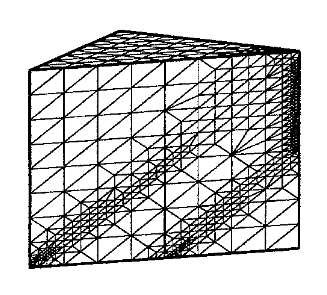
\includegraphics[width=0.75\textwidth]{inconsistent tessellation density.png}
    \caption{Illustration of inconsistent surface tessellation density (Bey, 1995).}
    \label{fig:inconsistenttess}
\end{figure}

\FloatBarrier

This approach has also been considered in relation to the original marching cubes algorithm. The adaptive marching cubes algorithm (Shu et al., 1995) takes a similar approach to Bey (1995) by subdividing some of the cubes within the sample volume, according to the curvature of the surface within each cube. A greater curvature will result in higher subdivision level, in order to preserve surface detail. Cubes are subdivided until the contained surface patch is considered sufficiently flat, or until a resolution limit is reached. This approach, like Bey (1995), balances high sample resolution with minimal triangle count and computational cost by effectively varying the sample resolution across the sample volume. One problem which this paper solves is the \textquotesingle crack problem\textquotesingle{} - when two neighbouring cubes have different degrees of subdivision, a crack may be produced in the resulting surface, due to one of the neighbours having a greater number of movable vertices on the shared face between them. Shu et al. propose a detection method for this, as well as a method to generate additional triangles to close the hole and maintain a watertight mesh.

A different approach presented by Labelle and Shewchuk (2007) fills the isosurface volumetrically with tetrahedra. This isosurface stuffing method is presented to guarantee a closed mesh in very minimal time; in fact the authors specifically note its applicability to real-time simulations. This technique guarantees dihedral angles - the angle between two facets in the resulting mesh - between 10.7° and 164.8°, helping to prevent sharp spikes or corners and making this method particularly applicable to extraction of smooth, organic surfaces. This is achieved by first excluding tetrahedra from the lattice which are not involved in the isosurface - i.e. which have no intersections - and then performing a modified form of marching tetrahedra, using the body-centered diamond lattice tessellation, where grid points may be warped if an edge\textquotesingle s intersection with the isosurface is determined to be too close to that grid point. The resulting tetrahedra are then sliced into several smaller tetrahedra using a set of pre-defined stencils, and the surfaces of these smaller tetrahedra become the final mesh surface as well as representing the volume profile of the mesh. This approach is able to generate reasonably regular meshes without need for any merging, as a result of how the underlying lattice grid is warped and tetrahedron edge cutting points are chosen. Its speed makes it useful for real-time applications such as videogames, however its implementation complexity makes it better suited for situations which benefit from deriving volume information about the isofunction.

Another category of approaches to isosurface extraction is dual contouring (Ju et al., 2002). Dual contouring requires information about the gradient of the function being sampled; a mesh is built by creating a single mesh element - usually a triangle or vertex - in each cell, and the joining these surface patches together with those in adjacent cells (Schaefer and Warren, 2004). The position of the mesh element is adapted within its cell to best fit the surface, a process which requires the ability to sample the gradient of the function being evaluated. This may present a need for significant additional computation, especially for functions defined by pre-sampled data such as medical imaging, where the gradient must be calculated by sampling adjacent data points. Otherwise, the technique allows significant room for adaptive simplification due to each cell only containing one mesh element. In addition, dual contouring lends itself well to GPU parallelisation (Hwang and Sung, 2024), which is potentially of great benefit for videogame terrain generation since many other computationally intensive components of game engines already take advantage of GPU compute shaders to parallelise data processing. As a related example, the Unity game engine supports evaluation of skinned mesh deformations in bulk using GPU compute shaders, enabling many skinned meshes to be rendered every frame (Unity Technologies, 2026).

In scenarios where geometry position and normal information is available, the gradient used by dual contouring can be inferred, making dual contouring a powerful tool for mesh reconstruction and simplification since it can efficiently sample mesh surface data and provides regularised mesh output by default. An implementation provided by Tao Ju is used by Blender\textquotesingle s \textquotesingle remesh\textquotesingle{} modifier (Bishop, 2011).

One example of the dual contouring method is the octree-based approach presented by Liang and Zhang (2013). This approach uses a similar strategy to Labelle and Shewchuk (2007) and Binninger et al. (2025) where grid points of the octree itself are adjusted in order to avoid producing small triangles. The octree is constructed with greater density around areas of the surface with higher curvature in order to preserve detail while minimising triangle count. While this approach is able to produce appropriately simplified meshes with good quality triangles, as has been already noted with other adaptive subdivision techniques, it results in an inconsistent level of detail, which is undesirable when applied to videogame terrain meshes.

The final major category of isosurface extraction techniques is the advancing front paradigm (Mueller, Roe, and Deconinck, 1992). This technique works by incrementally \textquotesingle growing\textquotesingle{} a triangulation across the isosurface, and is highly adaptable for different applications. It can be implemented to make use of gradient information when available, which can improve performance in scenarios where evaluating the gradient does not incur significant cost. Frey et al. (1998) propose a method for mesh extraction which combines Delaunay triangulation with the advancing front method to take advantage of the accurate point placement of the advancing front method.

Many authors have proposed improvements for the efficiency of the algorithm; Yu et al., (2022) introduce faster techniques for projecting candidate points onto the isosurface, and make use of an octree structure for identifying existing nodes to join frontal nodes with, resulting in an extremely fast sequential algorithm. Consideration has also been made in regard to parallelisation, particularly for the problem of balancing computational work between multiple computation units which may or may not share memory (Ito et al., 2007).

Overall, the advancing front method shows great potential for its surface adaptive nature - it does not suffer from marching cubes\textquotesingle{} problems with large regions of the sample being empty, wasting computation - as well as its ability to be integrated with other mesh construction techniques. In particular, it presents massively reduced memory consumption when compared to marching grid-based approaches.

\subsection{Mesh Simplification Techniques}\label{mesh-simplification-techniques}

As discussed in the introduction, isosurface extraction involves a run-time mesh generation step. Therefore, treating mesh simplification as a separate step nearly always increases overall computation time - even if the initial extraction step is less expensive. As such, simplifying as part of the mesh generation step is ideal from a performance perspective. However, it is useful to consider existing simplification techniques since they are an important point of comparison and may inform an integrated approach. This paper considers simplification methods specifically with regard to their ability to produce regularised results - meshes with near-equilateral, similar-area triangles - as well as preserve topology in the process.

One such technique is presented by Turk (1992). The algorithm is analogous to the constrained elastic surface nets extraction algorithm detailed above - points are distributed on the existing mesh surface, then repeatedly smoothed to produce an even distribution of new points while constraining them to lie on the original mesh. These new points are then combined with the original mesh in a "mutual tessellation", and this mesh is incrementally re-triangulated in localised patches to eliminate old vertices (see Fig. \ref{fig:retriangulation}) while preserving local surface topology. The result is an entirely re-tessellated, highly regularised mesh.

\begin{figure}[htb]
    \centering
    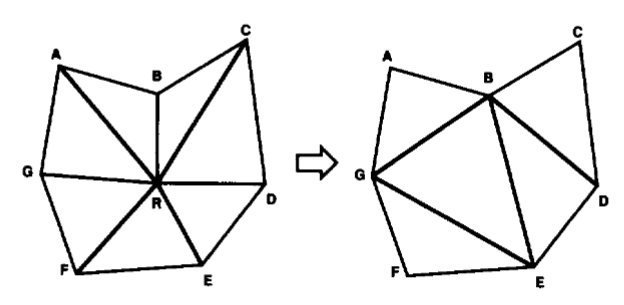
\includegraphics[width=0.75\textwidth]{local retriangulation.png}
    \caption{Example of a local re-triangulation to eliminate the vertex R (Turk, 1992).}
    \label{fig:retriangulation}
\end{figure}

\FloatBarrier

This technique could potentially be adapted to distribute points on an arbitrary mathematical surface - and in fact, this could be beneficial, providing a smooth surface defined at all points in space as well as curvature information by the use of derivatives - however, the problems of how to produce candidate points on the isosurface, and preserve topology without a guide mesh may present sufficient difficulty to discourage use of this approach.

One of the most efficient and trivial to implement simplification technique is vertex clustering. Naive vertex clustering simply groups vertices according to their proximity to their neighbours, and merges them together according to a distance threshold. However, this efficiency is gained by ignoring topological information, often resulting in topologically invalid (Cignoni et al., 1998) meshes - leading to holes and non-manifold surfaces. In addition, clustering often requires acceleration structures in order to efficiently search for nearby candidates for clustering, which also require computation to build and increase implementation complexity. The process of rebuilding the mesh at each step also becomes costly with large meshes, without topological information and additional complexity.

A similar technique is coplanarisation, which focuses on simplifying flat areas of a mesh. While this can be highly effective in some situations, it is not effective for organic, smoothly curved meshes and tends to produce highly irregular meshes (Cignoni et al., 1998), and thus is not applicable to the present use case.

A more advanced method for simplification is edge collapse. This approach begins by considering topology: a list of edges is first built using the list of triangles which define the mesh. These edges - pairs of vertices - are then checked individually, and are merged together if the edge length is less than a distance threshold. Finally, the mesh is reconstructed using the new vertex positions, discarding triangles which contain merged edges. Compared to vertex clustering, this technique eliminates a large number of wasted distance computations without the need for additional acceleration structures to be built. It also is more successful at preserving topology, although non-local topology - such as multi-edge loops covering a small area - is not always preserved. The edge collapse method also has a simple process for reconstructing the mesh, and does not require topology modifications between iterations of the edge length test. Because edges are merged one-by-one, this technique also produces highly regular meshes - demonstrated in section \ref{results-and-conclusions} - without additional vertex smoothing such as that used by the constrained elastic surface nets algorithm.

Another technique which may be of interest is octree hierarchical remeshing. This is a costly approach which works by representing the subject mesh as an octree - a three-dimensional, recursively subdivided structure, where each cell may be subdivided into eight half-sized cells. This octree is then un-subdivided by collapsing highly recursive octree cells, simplifying the representation of the mesh as a result. Finally, the octree can be used to construct a new mesh with a lower - potentially more consistent and regular - geometry density (Andújar et al., 1996).

\newpage

\section{Methodologies}\label{methodologies}

\subsection{Algorithm}\label{algorithm}

The implementation produced was based closely on the regularised marching tetrahedra algorithm (Treece, Prager, and Gee, 1999). However, several adaptations were made in order to produce ideal results for videogame terrain. The specific details of the algorithm developed are detailed below, beginning with the outline of the algorithm in pseudocode in Fig. \ref{fig:pseudocode}.

\begin{figure}[htb]
\begin{algorithm}[H]
\DontPrintSemicolon
Let $\mathbf{F}$ be a smoothly defined scalar function on $x,y,z$\;
Let $\mathbf{T}$ be the threshold value for which the isosurface is being computed\;
\For{each sample point in the lattice}{
	Let $\mathbf{P}$ be the position in space of the sample point\;
	Evaluate $\mathbf{F}$ for the given point $\mathbf{P}$, storing the result at the sample point\;
}
\For{each sample point in the lattice}{
	Let $\mathbf{C}$ equal the value of $\mathbf{F}$ at the current sample point\;
	Let $\mathbf{S1}\dots\mathbf{S14}$ equal the values of $\mathbf{F}$ at the neighbouring sample points in the lattice\;
	Let $\mathbf{I}$ be a series of Boolean flags representing isosurface intersections surrounding the current sample point\;
	\For{each neighbouring sample point}{
		\If{$sign(\mathbf{C}-\mathbf{T})\neq sign(\mathbf{S}n-\mathbf{T})$  \textbf{and} $\|\mathbf{C} - \mathbf{T}\| < \|\mathbf{S}n - \mathbf{T}\|$}{
			Set the flag in $\mathbf{I}$ corresponding to neighbour $n$\;
		}
    	}
	Store the value of $\mathbf{I}$ at the current sample point\;
	Using $\mathbf{I}$, construct a graph $\mathbf{G}$ representing which of these intersections can be merged together\;
	\uIf{$\mathbf{G}$ contains loops}{
		Skip to the next sample point\;
	}\Else{
		Check for disconnected islands in $\mathbf{G}$\;
		\For{each island in $\mathbf{G}$}{
			Create a single vertex $\mathbf{R}$ at the average position of all the isosurface intersections in the island\;
			Append $\mathbf{R}$ to the vertex array and let $\mathbf{V}$ be its index within the array\;
			\For{each intersection in the island}{
				Store $\mathbf{V}$ on the corresponding edge\;
			}
		}
	}
}
\For{each cube in the sample lattice}{
	Retrieve $\mathbf{I}$ from the sample point at the center of the cube\;
	\If{$\mathbf{I}$ has no flags set}{
		Skip to the next sample cube\;
	}
	// !TODO HERE!
}
\caption{Isosurface extraction}
\end{algorithm}
\caption{Pseudocode outlining the algorithm. The three \textbf{for} loops represent the three computation passes - sampling, vertex, and geometry generation.}
\label{fig:pseudocode}
\end{figure}

\FloatBarrier

!DIAGRAMS FOR THE WHOLE ALGORITHM 1xSAMPLING, 3xVERTEX, 2xGEOMETRY!

\subsubsection{Integrated Vertex Clustering Strategy}\label{integrated-vertex-clustering-strategy}

A novel approach to clustering vertices was developed. As discussed, the topology of the mesh should be preserved during merging, and thus the merging algorithm must behave differently depending on the topology. Based on the work of Treece, Prager, and Gee (1999), the only clustering considered is that of isosurface intersections which occur near a given sample point; sample points are processed one at a time. !DIAGRAM! This approach guarantees the algorithm to scale linearly on the number of sample points, and also prevents isosurface intersections from being involved in multiple merging operations, making the process order-independent and thus producing more consistent results. The topology is determined via a graph representation, and isosurface intersections are merged into vertices accordingly.  In this description, each sample point is surrounded by 14 neighbours, connected by edges. Each of these edges may have an isosurface intersection present, as indicated by the sample points at either end being in opposite states - where one is inside the isosurface, and the other outside. In this case, the position of the isosurface intersection can be calculated by linear interpolation along the edge; this is considered a \emph{\textquotesingle candidate vertex\textquotesingle}, since it may or may not represent a vertex in the final mesh. !DIAGRAM! If the candidate vertex is closer to the currently examined sample point than the neighbour, it is considered to be a \emph{\textquotesingle nearby intersection\textquotesingle{}} from the perspective of the currently examined sample point. The clustering and vertex creation processes operate on these nearby intersections only, with the understanding that distant intersections will be handled by the sample point to which they are nearest.

Hence, around each sample point, we have a set of nearby candidate vertices which may be able to be merged. The topology of this set must be considered, otherwise merging operations may be performed which compromise the topology of the resulting mesh. Several cases are demonstrated below: !DIAGRAM!

In each of these cases, the merging behaviour must be adjusted to preserve topology. Topology analysis is performed using an undirected graph (Bondy and Murty, 2008), represented using an adjacency matrix. This adjacency matrix is stored in the form of bitflags, since each nearby candidate vertex is either connected or unconnected to a given neighbour, and - since each sample point has 14 neighbours - at most 14 candidate vertices may be considered at a time. The use of bitflags both compacts the graph and makes it extremely fast to perform operations on, which is of great concern in this application. \emph{\textquotesingle Connections\textquotesingle{}} within the graph represent which pairs of edges between sample points - which may contain nearby candidate vertices - can be merged, which depends on two conditions: first, the edges must be adjacent to one another !DIAGRAM!; second, both the edges must have nearby candidate vertices.

Several topological features are then searched for using the graph. Before this stage begins, topologies where more than 10 nearby candidate vertices are present, merging is skipped, as this likely represents a complex, concave case. Next, the algorithm checks for the presence of loops. This is necessary to prevent unwanted collapsing of loops and preserve features like small tubes, which would otherwise fundamentally alter the topology of the mesh. Loops are detected by constructing a graph of all non-mergeable regions - the inverse of the graph described in the previous paragraph - and then searching for the presence of multiple islands. !DIAGRAM! If multiple islands are present in the inverted graph, then the un-inverted graph must therefore contain a loop, and thus merging is skipped for this sample point.

Next, disconnected regions or islands within the graph are identified. This must be performed in order to prevent separate, disconnected regions of the output mesh from being collapsed into one another. Islands are detected by progressively traversing the graph, marking traversed nodes with the current island number. When no more nodes are found to traverse, an unmarked node is searched for, the island number is incremented, and the process is repeated. When all nodes have been marked, the process is complete. From this the number of islands, and a 14-bit bitflag value for each, can be extracted. In order to preserve disconnected groups of nearby candidate vertices, each island is merged together independently.

Finally, mesh vertices are created according to the merging scheme deduced in the previous steps. References to these vertices - as indices into the vertex array - are stored on the appropriate edges between sample points. Reference to edge vertices are stored on the edge which corresponds to the candidate vertex in cases where it contributed to the given mesh vertex.

!FLOW DIAGRAM SHOWING THE WHOLE OF THIS PROCESS!

As explored in section \ref{technical-considerations}, the goal of this topology preservation is to ensure that the final mesh remains watertight and manifold. A non-watertight mesh would result in holes visible to the player; using an inappropriate merging scheme often leads to tight loops and fine details being lost, as well volumes being flattened into single triangles, resulting in non-manifold meshes with visible backfaces - single-sided geometry where both sides can be seen by the player.

The key limitation of our clustering technique is that it does not entirely guarantee preservation of manifoldness. Some cases of concave topology, or long and narrow islands, are not accounted for in the algorithm, and thus it is possible to produce single-sided geometry and collapsed loops in some topological cases. This could be resolved with extensions to the graph analysis process.

Overall, this localised merging approach is highly effective. It presents minimal cost due to the fixed maximum complexity of merging around a given sample point, as well as mostly preserving local topology. In addition, it avoids the need for potentially expensive vector distance calculations, instead preserving the distance threshold by virtue of considering candidate vertices locally around a particular sample point (thus the distance threshold must be between 1 - 2 times the resolution of the sample grid).

An alternative approach to solving the merging problem is a lookup table. This could be used to pre-compute the merging schemes for all candidate vertex configurations, simplifying runtime logic. However, a naive implementation would require a list of configurations of order $2^{14}$ or 16384, which - even if a merging scheme could be expressed in a single byte - would alone consume a quarter of the entire L1 cache in a typical desktop CPU (TechPowerUp, \emph{AMD Ryzen 5 3600 Specs}). This would likely lead to a high frequency of cache misses, significantly slowing down this critical part of the algorithm. As such, an on-the-fly graph theory approach was taken, which also allows for non-constant completion time via early escape from particular topology configurations where merging is not possible.

\subsubsection{Optimisation Considerations}\label{optimisation-considerations}

The arrangement of computation passes was arranged with intent to minimise execution time. A major challenge when implementing the algorithm was efficient data access. In order to reduce the number of memory accesses performed, the process of identifying isosurface intersections with lattice edges and the process of merging and computing vertex positions were merged into a single \emph{\textquotesingle vertex\textquotesingle{}} pass. This eliminates a large amount of storing and retrieving of information which can instead be made local within the combined vertex pass, as well as reducing the overall memory usage of the algorithm.

During the vertex and geometry passes, access to neighbouring sample points is required. Access to these is accelerated by keeping a table of offsets which, when added to the array index of the current sample point, produce the index of the neighbour point corresponding to a given direction. This is also performed for the spatial vectors between sample points to avoid recomputation many times over. !DIAGRAM!

Further optimisations are made by using the proximity flags to determine where there is one or fewer nearby intersections to skip the clustering process. Similarly, when the geometry pass encounters a cube where the intersection flags value is zero, the entire cube - consisting of 24 tetrahedra - is skipped, since this indicates that no geometry is present in the relevant tetrahedra; this massively reduces the processing cost of this step. This mirrors the work of Bajaja et al. (1996) - discussed earlier - to reduce the amount of computation required for a given sample volume by filtering out cells which have no isosurface intersections.

Another alteration made to the Treece, Prager, and Gee (1999) algorithm is that in the current implementation, vertex normal vectors are calculated naively without evaluating surface curvature. This decision was made to reduce the computational cost of the algorithm and thus improve overall performance. Normal vectors are instead calculated by computing the mean interpolated normal vector for attached triangles after geometry has been generated. This also guarantees more appropriate shading for use in the context of videogames, as players are less concerned with the accuracy of the surface shading to the underlying noise function, and more so whether the terrain looks smooth and avoids shading artefacts.

\subsubsection{Tetrahedral Arrangements}\label{tetrahedral-arrangements}

Two methods for tessellating space using tetrahedra are tested. The first of which is that recommended by other works, including Treece, Prager, and Gee (1999), the body-centered diamond lattice structure, shown in !DIAGRAM!. This arrangement consists of 24 tetrahedra per lattice cube, although each of these tetrahedra is shared between two cubes, so the effective number per lattice cube is 12. The arrangement is highly desirable, since it is symmetric in many axes and contains near-regular tetrahedra as described in section \ref{marching-tetrahedra}.

The second method is the \emph{\textquotesingle simple cubic\textquotesingle{}} arrangement, similar to that described by Chan and Purisima (1998). The tetrahedra are entirely contained within a cube, which is sliced first along the diagonal axis, then along each of the cube faces. Cuts are made in the same direction for opposing cube faces, which eliminates the need to mirror the layout of each alternating cube in the resulting lattice and thus simplifies the implementation. These cuts are then joined into 6 tetrahedra within the cube, each with two external faces !DIAGRAM!. This modified arrangement has the advantage - against the original simple cubic arrangement presented by Chan and Purisima - that all tetrahedra are geometrically congruent, making the produced triangles more consistent in size.

However, this arrangement suffers from two key issues, which are the irregularity of the tetrahedra - dihedral angles are not consistent between faces, and are far from the 90 degrees of regular tetrahedra, as well as having an overall aspect ratio considerably above 1; and the directional bias - the fact that all tetrahedra share a central axis leads to limited freedom of movement for vertices created using the lattice, resulting in a directional bias sometimes visible in the final mesh.

Both tessellations are structured such that each sample point has 14 connected neighbours - excluding points on the outer faces of the sample volume. This makes implementation of the two approaches simple and enables per-edge Boolean information to be stored in a single 16-bit value per sample point.

\subsubsection{Parallelisation Approach}\label{parallelisation-approach}

The original RMT algorithm does not take advantage of CPU parallelisation. However, parallelisation capability of CPUs is abundant on modern hardware, which can be taken advantage of. The implementation provides parallelisation capability for the sampling pass only, where the number of worker threads is specified by the user. The decision to limit the parallelisation was taken based on measurements taken for the duration of different areas of the algorithm. It was found that the vast majority of the computation time for the algorithm was spent evaluating the user-provided sample function; this is reflected in the section \ref{results-and-conclusions}.

Another candidate for multi-threading support was the vertex generation pass, which involves most of the remaining computation work for the algorithm, due to the clustering procedure. However, since this process involves appending vertices to a shared list - and more importantly, maintaining a unique index referencing each - difficulties arise when refactoring the algorithm for parallel processing. Avoiding extensive use of synchronisation primitives (mutices) requires a non-trivial process of merging the outputs from multiple threads, which itself can be extremely costly in addition to the limitations imposed by Amdahl\textquotesingle s law (Hill and Marty, 2008). As such the decision was made not to parallelise this aspect of the algorithm. !DIAGRAM OF AN EXAMPLE PARALLELISATION METHOD, THE GOOD ONE I CAME UP WITH!

In addition, the consideration is made below that the user may wish to divide the sample volume into chunks, and that these chunks may be processed in parallel. Thus, it may be beneficial to limit the resource usage of a single instance of the algorithm in order to facilitate user-controlled forms of parallelisation without exhausting CPU parallelisation capacity.

\subsection{Evaluation}\label{evaluation}

\subsubsection{Comparisons of Interest}\label{comparisons-of-interest}

In comparing different mesh generation approaches, the measurable factors of interest are as follows:
\begin{itemize}
\tightlist
\item The time taken to produce the mesh
\item The number of triangles in the resulting mesh, and thus the rendering cost
\item The triangle quality of the resulting mesh, and thus the visual quality perceived by players
\end{itemize}
In particular, consideration is made in terms of visual quality per arbitrary performance unit, since videogame terrain generation must balance the experience of players with the cost of delivering that experience.
\\
\\
Three variables are tested in the evaluation of the algorithms:
\begin{itemize}
\tightlist
\item The sample object; a sphere, an asteroid shape produced by a procedural noise function, and the Stanford \textbf{Bunny} (Turk and Levoy, 1994)
\item The tetrahedron arrangement; body-centered diamond lattice, or simple cubic
\item The clustering method; no clustering, integrated clustering, or post-processed merging using edge collapse
\end{itemize}
Every configuration of these variables is evaluated in both the benchmark and questionnaire processes, which results in 18 different test cases overall:
\begin{itemize}
\tightlist
\item Sphere object; body-centered arrangement; no clustering
\item Sphere object; body-centered arrangement; integrated clustering
\item Sphere object; body-centered arrangement; post-processed clustering
\item Sphere object; simple arrangement; no clustering
\item Sphere object; simple arrangement; integrated clustering
\item Sphere object; simple arrangement; post-processed clustering
\item Asteroid object; body-centered arrangement; no clustering
\item Asteroid object; body-centered arrangement; integrated clustering
\item Asteroid object; body-centered arrangement; post-processed clustering
\item Asteroid object; simple arrangement; no clustering
\item Asteroid object; simple arrangement; integrated clustering
\item Asteroid object; simple arrangement; post-processed clustering
\item Bunny object; body-centered arrangement; no clustering
\item Bunny object; body-centered arrangement; integrated clustering
\item Bunny object; body-centered arrangement; post-processed clustering
\item Bunny object; simple arrangement; no clustering
\item Bunny object; simple arrangement; integrated clustering
\item Bunny object; simple arrangement; post-processed clustering
\end{itemize}

!SHOULD THESE BE AN APPENDIX INSTEAD?!

\subsubsection{Benchmarking}\label{benchmarking}

The implementation was profiled numerically for the configurations described above with regard to several metrics:
\begin{itemize}
\tightlist
\item The time taken to produce the mesh, including the percentage of time spent in each step - sampling, vertex creation, geometry creation, normal computation
\item The mean aspect ratio of triangles in the resulting mesh, as a quantitative measure of the quality of resulting shading
\item The number of triangles and vertices in the resulting mesh
\end{itemize}
Each benchmark was performed 100 times to account for background variations in CPU load and other conditions, and the mean value of each metric is then computed. The tests were performed on an \texttt{HP Z2 G8 Tower Workstation Desktop PC} running \texttt{Windows 11 Enterprise 24H2}, and consisting of an \texttt{11th Gen Intel Core i7-11700 CPU @2.5GHz with 16 Logical processors, 640KB L1 cache, 4MB L2 cache, 16MB L3 cache; and 32GB of 3200MT/s DDR4 RAM}.

\subsubsection{Questionnaire}\label{questionnaire}

The perceived visual quality of a mesh is assessed using a questionnaire. Each question consists of a pair of animations playing side- by-side, where each animation shows the mesh resulting from a different configuration of the test variables. The participant is then asked which of the two animations they prefer, selecting from \textquotesingle Prefer left\textquotesingle, \textquotesingle No preference\textquotesingle, or \textquotesingle Prefer right\textquotesingle.

Variables are tested independently to isolate their impact from one another, and due to restrictions on time for collecting user feedback data. This means that only one parameter differs between the animations in a given question - for example, the clustering method may be switched between the left and right animations. Additionally, animations may only be compared if both animations use the same sample object, since there is no need to compare the visual quality between different sample meshes with otherwise the same parameters.

Ideally, each pair of animations (and thus configurations) would be shown in two separate questions, reversed in the second occurrence - for every question showing animations \textbf{A} and \textbf{B}, there would be a corresponding question showing animations \textbf{B} and \textbf{A}. This would reduce the potential bias introduced by participants having an inherent left or right preference; however this would double the length of the questionnaire, potentially increasing the prevalence of issues discussed below.

The questionnaire consists of 27 questions, and the specific comparisons made are shown in !INCLUDE QUESTIONNAIRE AS AN APPENDIX!. The length of the questionnaire is of significance - due to the data collection depending on a volunteer sampling method, and there being no incentive to participate, a questionnaire which takes a long time to complete will likely deter possible  participants, reducing the size of the dataset. In addition, longer completion times may lead to participants developing fatigue during the questionnaire and paying less attention to later questions as a result, in order to reach the end quicker, also reducing the reliability of the resulting data.

In order to obscure the configurations involved in any given question - to blind the participants - animation files are named using non-indicative 4-letter names, and questions are simply titled according to their number. In addition, questions are presented in a randomised order to deter participants from identifying and kind of pattern with the animations. This randomisation also helps to reduce the potential effect of fatigue, as participants will not all see the same questions last.

Animations for the questionnaire are generated by an additional tool built into the implemented artefact which automatically produces a GIF animation of the generated mesh rotating in space. All parameters for the creation of the GIF, such as length, framerate, resolution, and camera angle, are kept the same between different animations to eliminate confounding variables. GIF files are then paired up, upscaled by a factor of 2 using nearest-point interpolation, and combined side-by-side into video files using the command-line tool FFMPEG. Each resulting video file is named based on the two animations it consists of, using the same non- indicative 4-letter naming convention, for use when assembling the questionnaire and results.

The results are analysed using a system of preference points, which are weighted within their individual comparison groups to determine the relative preference of each configuration of test variable. These are then combined with the preference weights from other comparison groups using an arithmetic mean.

\section{Results and Conclusions}\label{results-and-conclusions}

!SIZE OF DATASET! !CONFIDENCE INTERVAL OR WHATEVER? p=0.05!

\section{Bibliography}\label{bibliography}

Che, L. \emph{et al.} (1985) `Surface shading in the Cuberille
environment', \emph{IEEE Computer Graphics and Applications}, 5(12), pp.
33--43. doi:10.1109/mcg.1985.276275.\\
Lorensen, W.E. and Cline, H.E. (1998) `Marching cubes', \emph{Seminal
graphics}, pp. 347--353. doi:10.1145/280811.281026.\\
Chan, S.L. and Purisima, E.O. (1998) `A new tetrahedral tesselation
scheme for isosurface generation', \emph{Computers \& Graphics}, 22(1),
pp. 83--90. doi:10.1016/s0097-8493(97)00085-x.\\
Chan, S.L. and Purisima, E.O. (1998) \textquotesingle Molecular surface
generation using marching tetrahedra\textquotesingle, \emph{Journal of
Computational Chemistry}, 19(11) pp. 1268-1277.
doi:10.1002/(SICI)1096-987X(199808)19:11\%3C1268::AID-JCC6\%3E3.0.CO;2-I\\
Treece, G.M., Prager, R.W. and Gee, A.H. (1999) `Regularised marching
tetrahedra: Improved iso-surface extraction', \emph{Computers \&
Graphics}, 23(4), pp. 583--598. doi:10.1016/s0097-8493(99)00076-x.\\
Zhou, Y., Chen, W. and Tang, Z. (1995) `An elaborate ambiguity detection
method for constructing isosurfaces within tetrahedral meshes',
\emph{Computers \& Graphics}, 19(3), pp. 355--364.
doi:10.1016/0097-8493(95)00006-x.\\
Gallagher, R.S. and Nagtegaal, J.C. (1989) `An efficient 3-D
visualization technique for finite element models and other coarse
volumes', \emph{ACM SIGGRAPH Computer Graphics}, 23(3), pp. 185--194.
doi:10.1145/74334.74352.\\
Nielson, G.M. and Hamann, B. (1991) `The asymptotic decider: Resolving
the ambiguity in Marching Cubes', \emph{Proceeding Visualization '91}
{[}Preprint{]}. doi:10.1109/visual.1991.175782.\\
Sun, H. \emph{et al.} (2023) `Multi-labeled regularized marching
tetrahedra method for implicit geological modeling', \emph{Mathematical
Geosciences}, 56(2), pp. 219--248. doi:10.1007/s11004-023-10075-9.\\
Bajaj, C.L., Pascucci, V. and Schikore, D.R. (1996) `Fast isocontouring
for improved interactivity', in \emph{Proceedings of the 1996 Symposium
on Volume Visualization}. San Francisco, California, USA: IEEE Press
(VVS '96), pp. 39-ff.
\url{https://dl.acm.org/doi/10.5555/236226.236231}\\
Gibson, S.F. (1998) `Constrained elastic surface nets: Generating smooth
surfaces from binary segmented data', \emph{Lecture Notes in Computer
Science}, pp. 888--898. doi:10.1007/bfb0056277.\\
Lee, J.M. (2012) `Smooth Manifolds', in \emph{Introduction to smooth
manifolds}. Springer Nature, pp. 1--31.\\
Penner, E. (2011) `VI, 2.3 Pixel Derivatives and Pixel Quads', in W.
Engel (ed.) \emph{GPU pro 2: Advanced rendering techniques}. New York:
Taylor \& Francis, pp. 350--352.\\
Payne, B.A. and Toga, A.W. (1990) `Surface mapping brain function on 3D
models', \emph{IEEE Computer Graphics and Applications}, 10(5), pp.
33--41. doi:10.1109/38.59034.\\
Binninger, A. \emph{et al.} (2025) `Tetweave: Isosurface extraction
using on-the-fly Delaunay tetrahedral grids for gradient-based mesh
optimization', \emph{ACM Transactions on Graphics}, 44(4), pp. 1--19.
doi:10.1145/3730851.\\
Qiu, Z. \emph{et al.} (2024) `Deformable Nerf using recursively
subdivided tetrahedra', \emph{Proceedings of the 32nd ACM International
Conference on Multimedia}, pp. 6424--6432.
doi:10.1145/3664647.3681019.\\
Bey, J. (1995) `Tetrahedral grid refinement', \emph{Computing}, 55(4),
pp. 355--378. doi:10.1007/bf02238487.\\
Turk, G. (1992) `Re-tiling polygonal surfaces', \emph{Proceedings of the
19th annual conference on Computer graphics and interactive techniques},
pp. 55--64. doi:10.1145/133994.134008.\\
Cignoni, P., Montani, C. and Scopigno, R. (1998) `A comparison of mesh
simplification algorithms', \emph{Computers \& Graphics}, 22(1), pp.
37--54. doi:10.1016/s0097-8493(97)00082-4.\\
Andújar, C. \emph{et al.} (1996) `Automatic generation of
multiresolution boundary representations', \emph{Computer Graphics
Forum}, 15(3), pp. 87--96. doi:10.1111/1467-8659.1530087.\\
Shu, R., Zhou, C. and Kankanhalli, M.S. (1995) `Adaptive Marching
cubes', \emph{The Visual Computer}, 11(4), pp. 202--217.
doi:10.1007/bf01901516.\\
Labelle, F. and Shewchuk, J.R. (2007) `Isosurface stuffing', \emph{ACM
SIGGRAPH 2007 papers}, p. 57. doi:10.1145/1275808.1276448.\\
Castelo, A. \emph{et al.} (2024) `A generalized combinatorial marching
hypercube algorithm', \emph{Computational and Applied Mathematics},
43(3). doi:10.1007/s40314-024-02627-4.\\
Liang, X. and Zhang, Y. (2013) `An octree-based dual contouring method
for triangular and tetrahedral mesh generation with guaranteed angle
range', \emph{Engineering with Computers}, 30(2), pp. 211--222.
doi:10.1007/s00366-013-0328-8.\\
Schaefer, S. and Warren, J. (2004) `Dual Marching Cubes: Primal
contouring of dual grids', \emph{12th Pacific Conference on Computer
Graphics and Applications, 2004. PG 2004. Proceedings.}, pp. 70--76.
doi:10.1109/pccga.2004.1348336.\\
\emph{AMD Ryzen 5 3600 Specs} (no date) \emph{TechPowerUp}. Available
at: \url{https://www.techpowerup.com/cpu-specs/ryzen-5-3600.c2132}
(Accessed: 10 February 2026).\\
Raffe, W.L., Zambetta, F. and Li, X. (2012) `A survey of procedural
terrain generation techniques using evolutionary algorithms', \emph{2012
IEEE Congress on Evolutionary Computation}, pp. 1--8.
doi:10.1109/cec.2012.6256610.\\
\emph{ASTRONEER}. (2016). PC {[}Game{]}. Seattle, Washington: System Era
Softworks.\\
Hwang, J. and Sung, M. (2024) `Occupancy-based dual contouring',
\emph{SIGGRAPH Asia 2024 Conference Papers}, pp. 1--11.
doi:10.1145/3680528.3687581.\\
Ju, T. \emph{et al.} (2002) `Dual contouring of Hermite Data',
\emph{Proceedings of the 29th annual conference on Computer graphics and
interactive techniques}, pp. 339--346. doi:10.1145/566570.566586.\\
Bishop, N. (2011) \emph{Remesh modifier}, \emph{Blender Developers
Blog}. Available at:
\url{https://code.blender.org/2011/12/remesh-modifier/} (Accessed: 10
February 2026).\\
Mueller, J.-D., Roe, P.L. and Deconinck, H. (eds) (1992) \emph{A frontal
approach for node generation in Delaunay triangulations}.\\
Frey, P.J., Borouchaki, H. and George, P.-L. (1998) `3D Delaunay mesh
generation coupled with an advancing-front approach', \emph{Computer
Methods in Applied Mechanics and Engineering}, 157(1--2), pp. 115--131.
doi:10.1016/s0045-7825(97)00222-3.\\
Yu, K. \emph{et al.} (2022) `On the efficiency of the advancing-front
surface mesh generation algorithm', \emph{Computer-Aided Design}, 153,
p. 103403. doi:10.1016/j.cad.2022.103403.\\
Ito, Y. \emph{et al.} (2007) `Parallel unstructured mesh generation by
an advancing front method', \emph{Mathematics and Computers in
Simulation}, 75(5--6), pp. 200--209. doi:10.1016/j.matcom.2006.12.008.\\
Delaunay, B. (1934) `Sur la sphère vide', \emph{Bulletin de l'Académie
des Sciences de l'URSS. VII. Série}, 1934(6), pp. 793--800.\\
\emph{MeshDeformation GPUBatched} (2026) \emph{Unity Documentation}.
Available at:
\url{https://docs.unity3d.com/6000.0/Documentation/ScriptReference/MeshDeformation.GPUBatched.html}
(Accessed: 15 February 2026).\\
Bondy, J.A. and Murty, U.S.R. (2008) \emph{Graph theory}. New York:
Springer.\\
Hill, M.D. and Marty, M.R. (2008) `Amdahl's Law in the Multicore Era',
\emph{Computer}, 41(7), pp. 33--38. doi:10.1109/mc.2008.209.\\
Turk, G. and Levoy, M. (1994) `Stanford Bunny'. Stanford University
Computer Graphics Laboratory.

\end{document}
